\documentclass[USenglish]{article}

\usepackage{ifikompendiumforside}
\usepackage{graphicx}
\usepackage[acronym]{glossaries}
\makeglossaries

% Acronyms
\newacronym{dil}{DIL}{Disconnected, Intermittent and Limited environments}

\title{Improving the performance of Web Services in Disconnected, Intermittent and Limited Environments}
\author{Joakim Johanson Lindquister}

\begin{document}
\ififorside{}

\begin{abstract}
    My abstract
\end{abstract}

\part{Introduction}
Kort intro om oppgaven her.
\section{Background and Motivation}
Hvorfor?

\section{Problem Statement}
Most of the Web Service solutions used today are aimed for civilian use and does
not necessarily perform well in military environments. In contrast to civilian
networks where bandwidth are abundant, mobile tactical networks may suffer
from high error rates and low bandwidth.

In my master thesis I will investigate different optimization techniques that
can be applied to improve communication. In order for the clients and services
 to remain interoperable the optimization techniques will be placed in proxies.

The Web Services will communicate with his counter part over HTTP as regular,
with all traffic going umerkelig through the proxy. The Web Service itself does
not need to pay attention to the bad connectivity, the proxy will choose the
appropriate protocol and configuration.

\section{Premises}
Ikke endre web-servicene.

\section{Scope and Limitations}
Snevre inn oppgaven

\section{Research Methodology}

\section{Contribution}
Hva er det oppgaven min bidrar med?
\section{Outline}
Hvordan er resten av oppgaven strukturert.


\part{Background}
\section{Related Work}
Diskuterer eksisterende arbeid.

\section{Requirement Analysis}

\section{DIL}
\gls{dil} definer hva DIL er og hvilke begrensninger det legger.

\section{Summary}

\part{Design and Implementation}
\section{Overall Design}
\section{Proxy}
\subsection{Squid}
Squid is a fully-featured HTTP/1.0 proxy.
\begin{figure}[h]
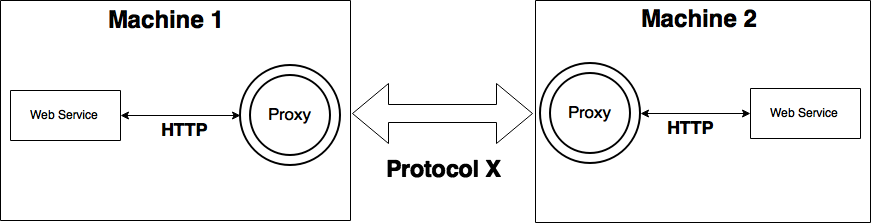
\includegraphics[scale=0.4]{images/architecture.png}
\caption{Architectural overview of proposed design}
\end{figure}

\section{Summary}

\part{Testing and Evaluation}
\section{Evaluation Tools}

\part{Conclusion and Future Work}
\section{Conclusion}

\section{Future Work}



\printglossary

\end{document}
